\documentclass[12pt, a4paper]{article}
\input{/home/mykhailo/.config/nvim/templates/preamble.tex}

\newcommand{\department}{ЗІ}
\newcommand{\reportnumber}{3}
\newcommand{\reporttitle}{Робота з CSS}
\newcommand{\profname}{Синявський О. Ю.}

\begin{document}

\input{/home/mykhailo/Documents/lpnu/report_title_page}

\section{Частина 1. Вступ до CSS}
Мета --- опанувати основні принципи стилізації вебсторінок за допомогою CSS. Ознайомитися з методами підключення каскадних таблиць стилів (вбудовані, внутрішні, зовнішні). Навчитися використовувати різні селектори (селектори тегів, класів, ID, атрибутів, псевдокласів). Зрозуміти концепцію "Box Model" та основи побудови макетів за допомогою Flexbox або Grid Layout.
\subsection{Хід роботи}
\begin{enumerate}
	\item Створіть файл з назвою style.css.
	\item Підключіть цей файл до файлу index.html з попередньої лабораторної роботи.
	\item Оформіть сторінку за допомогою CSS. Результат має містити щонайменше:
		\begin{itemize}
			\item Усі три способи підключення стилів по одному разу (inline, internal, external), причому основна частина правил лежить у зовнішньому файлі.
			\item Селектори тегів, класів, ID та атрибутів, а також щонайменше два псевдокласи.
			\item Явне керування блоковою моделлю margin, padding, border та box-sizing.
			\item Макет сторінки, побудованих на Flexbox або CSS Grid, а не на float.
			\item Медіазапит, який змінює макет на вузькому екрані.
		\end{itemize}
\end{enumerate}
\subsection{Лістинг}
\textbf{index.html}
\begin{lstlisting}
<!DOCTYPE html>
<html>
	<head>
		<title>CV - Кохманський Михайло</title>
		<link rel="stylesheet" href="styles.css">
		<style>		
			*, *::before, *::after {
			  box-sizing: border-box;
			}

			body, h1, h2, h3, h4, h5, h6, p, figure, blockquote, dl, dd {
			  margin: 0;
			}

			html {
			  color-scheme: light dark;
			}

			body {
			  min-height: 100vh;
			  line-height: 1.5;
			  font-family: system-ui, -apple-system, sans-serif;
			}

			img, picture, video, canvas, svg {
			  display: block;
			  max-width: 100%;
			}

			input, button, textarea, select {
			  font: inherit;
			}

			p, h1, h2, h3, h4, h5, h6 {
			  overflow-wrap: break-word;
			}

			p {
			  text-wrap: pretty;
			}
			h1, h2, h3, h4, h5, h6 {
			  text-wrap: balance;
			}
		</style>
	</head>
	<body>
		<div id="outerWrapper">
			<div id="innerContainer">
				<header>
					<div id="headerWrapper">
						<div id="infoContainer">
							<h1 id="name" style="color: #fff" >Кохманський Михайло Михайлович</h1>
							<p id="specialization">Information security specialist</p>
							<p id="city">Місто: Львів, Україна</p>
						</div>
						<div id="headerButtons">
							<a
								href="mailto:mykhailo.kokhmanskyi.kb.2025@lpnu.ua"
								id="emailHref"
								class="button"
							>
            					Email
							</a>
							<a
								href="https://github.com/MykhailoKokhmanskyi"
								target="_blank"
								rel="noopener noreferrer"
								id="githubHref"
								class="button"
							>	
        					    GitHub
							</a>
						</div>
					</div>
				</header>
				<main>
					<section id="about">
						<h2>Про мене</h2>
						<p>
							Я студент спеціальності "Кібербезпека", який захоплюється вивченням методів захисту інформаційних систем, аналізом вразливостей та мережевою безпекою. Активно розвиваю практичні навички в тестуванні на проникнення, безпеці вебдодатків та криптографії, а також регулярно беру участь у CTF-змаганнях. Прагну застосувати отримані знання в реальних проектах для виявлення загрози та побудови надійних систем захисту даних.
						</p>
					</section>
					<section id="skills">
						<h2>Навики</h2>
						<div id="skillContainer">
							<div id="languagesContainer" class="skillCategory">
								<h3>Мови програмування</h3>
								<div class="skillItemContainer">
									<span class="skillItem">HTML</span>
									<span class="skillItem">CSS</span>
									<span class="skillItem">JavaScript</span>
									<span class="skillItem">Python3</span>
									<span class="skillItem">Lua</span>
								</div>
							</div>
							<div id="librariesContainer" class="skillCategory">
								<h3>Бібліотеки і фреймворки</h3>
								<div class="skillItemContainer">
									<span class="skillItem">React.js</span>
									<span class="skillItem">Express.js</span>
									<span class="skillItem">Next.js</span>
									<span class="skillItem">JWT</span>
								</div>
							</div>
							<div id="toolsContainer" class="skillCategory">
								<h3>Інструменти</h3>
								<div class="skillItemContainer">
									<span class="skillItem">Git</span>
									<span class="skillItem">GitHub</span>
									<span class="skillItem">Vim</span>
									<span class="skillItem">Linux</span>
									<span class="skillItem">LaTeX</span>
									<span class="skillItem">SQL</span>
									<span class="skillItem">MySQL</span>
									<span class="skillItem">PostgreSQL</span>
									<span class="skillItem">MongoDB</span>
									<span class="skillItem">SSL</span>
									<span class="skillItem">SSH</span>
								</div>
							</div>
						</div>
					</section>
					<section id="projects">
						<h2>Проекти</h2>
						<article id="lpmonitor">
							<div id="projectHeader">
								<h3>LPMonitor <span class="muted">- Платформа краудсорсингового моніторингу сервісів</span></h3>
								<span id="delayed">Проект відкладено</span>
							</div>

							<div id="skillContainer">
								<span class="skillItem">Node.js</span>
								<span class="skillItem">Express.js</span>
								<span class="skillItem">AWS (Lightsail, SES)</span>
								<span class="skillItem">HTML</span>
								<span class="skillItem">SSR</span>
								<span class="skillItem">PostgreSQL</span>
							</div>
							<div id="linksContainer">					
								<a href="https://lpmonitor.org" class="projectLink">Live Demo</a>
								<a href="https://github.com/MykhailoKokhmanskyi/LPMonitor" class="projectLink">GitHub Repository</a>
							</div>
							<ul id="projectDetails">
								<li>Розробив та розгорнув прототип системи моніторингу доступності університетських серввісів на основі краудсорсингу.</li>
								<li>Реалізував базову систему автентифікації користувачів та проміжне програмне забезпечення (middleware) для обробки запитів.</li>
								<li>Налаштував обмеження частоти запитів (Rate Limiting) для захисту сервера від перевантаження та зловживань.</li>
								<li>Налаштував хостинг серверного вебдодатка (SSR) на базі AWS Lightsail, керування DNS-записами та інтегрував AWS SES для надсилання електронних листів для підтвердження електронної адреси.</li>
							</ul>
						</article>
					</section>
					<section id="education">
						<h2>Освіта</h2>
						<article class="skillCategory between">
							<div>
								<h3>F5 - Кібербезпека</h3>
								<p>Національний Університет "Львівська Політехніка"</p>
							</div>
							<span>2025-2029</span>
						</article>
					</section>
				</main>
				<footer><p>&copy; 2026 Кохманський Михайло. Всі права захищено.</p></footer>
			</div>
		</div>
	</body>
</html>
\end{lstlisting}

\textbf{styles.css}
\begin{lstlisting}
#outerWrapper {
	min-height: 100vh;
	background: #020618;
	text: #f1f5f9;
	font-family: Sans-Serif;
	padding: 1rem 2.5rem;
}

#innerContainer {
	max-width: 56rem;
	margin: 0 auto;
	background: #0f172b;
	border-radius: 1rem;
	border: #1e293b 1px solid;
	padding: 1.5rem;
	overflow: hidden;
}

#innerContainer > * + * {
	margin-top: 2rem;
}

header {
	border-bottom: 1px solid #1e293b;
	padding-bottom: 2rem;
}

#headerWrapper {
	display: flex;
	flex-direction: column;
	justify-content: space-between;
	align-items: flex-start;
	gap: 1rem;
	width: fit-content;
}

#infoContainer {
	width: fit-content;
}

#name {
	font-size: 2rem;
	width: 36rem;
	font-weight: bold;
}

#specialization {
	font-size: 1rem;
	width: fit-content;
	font-weight: 500;
	color: #34d399;
}

#city {
	font-size: 0.8rem;
	color: #90a1b9;
	width: fit-content;
}

#headerButtons {
	display: flex;
	flex-direction: column;
	gap: 0.75rem;
	font-size: 0.8rem;
}

.button {
	padding: 0.5rem 1rem;
	color: white;
	border-radius: 0.5rem;
	transition: 0.3s;
	text-decoration: none;
}

#emailHref {
	background-color: #1E293B;
	border: 1px solid #334155;
}

#emailHref:hover {
	background-color: #334155;
}

#githubHref {
	background-color: #009669;
}

#githubHref:hover {
	background-color: #00bc7d;
}

@media(min-width: 640px) {
	#outerWrapper {
		padding: 1rem 1.5rem;
	}

	#innerWrapper {
		padding: 2.5rem;
	}

	#headerButtons {
		flex-direction: row;
	}
}

main > * + * {
	margin-top: 2.5rem;
}

main section > * + * {
	margin-top: 0.75rem;
}

main section h2 {
	font-size 1.75rem;
	font-weight: 500;
	color: #E2E8F0;
	border-left: 4px solid;
	border-color: #10B981;
	padding-left: 0.75rem;
}

section#about p {
	color: #CBD5E1;
	font-size: 1.25rem;
}

#skillContainer > * + * {
	margin-top: 0.75rem;
}

.skillCategory {
	background: #020617;
	padding: 1.5rem;
	border-radius: 0.75rem;
	border: 1px solid #1D293D;
	transition: 0.3s;
}
.skillCategory h3 {
	font-size:0.75rem;
	text-transform: uppercase;
	font-weight: 500;
	margin-bottom: 0.5rem;
	color: #93A3B8;
}
.skillItemContainer {
	display: flex;
	flex-wrap: wrap;
	gap: 0.5rem;
}
.skillItem {
	background: #1e293b;
	color: #93a3b8;
	font-size: 0.75rem;
	padding: 0.25rem 0.5rem;
	border-radius: 0.25rem;
	border: 1px solid #334155;
}

.skillCategory:hover {
	border: 1px solid #334155;
}

#lpmonitor {
	background: #020617;
	padding: 1.5rem;
	border-radius: 0.75rem;
	border: 1px solid #1e293b;
	transition: 0.3s;
}
#lpmonitor:hover {
	border: 1px solid #334155;
}
#projectHeader {
	display: flex;
	flex-direction: column;
	justify-content: space-between;
	align-items: flex-start;
	gap: 0.5rem;
	margin-bottom: 0.75rem;
}
#projectHeader h3 {
	font-size: 1.5rem;
	max-width: 36rem;
	font-weight: bold;
}
.muted {
	color: #94a3b8;
	font-weight: normal;
}
#delayed {
	background: #F59E0B1A;
	color: #FBBF24;
	border: 1px solid #F59E0B33;
	font-size: 0.75rem;
	font-weight: 500;
	padding: 0.25rem 0.5rem;
	border-radius: 0.25rem;
}

#linksContainer {
	display: flex;
	gap: 1rem;
	font-size: 0.75rem;
	font-weight: 500;
	margin: 0.75rem;
}

.projectLink {
	text-decoration: none;
	color: #34D399;
}
.projectLink:hover {
	text-decoration: underline;
}

#projectDetails {
	list-style-type: disc;
	list-style-position: inside;
}
#projectDetails li::marker {
	color: #10B981;
}
#education h3 {
	color: white;
	font-size: 1rem;
	font-weight: bold;
}

#education p {
	color: #94a3b8;
	font-size: 0.75rem;
}

.between {
	display: flex;
	flex-direction: row;
	justify-content: space-between;
	align-items: center;
}
#education span {
	font-size: 0.5rem;
	font-weight: 500;
	color: #34d399;
	background-color: #022c2266;
	border: 1px solid #065f46;
	border-radius: 100rem;
	padding: 0.25rem 0.75rem;
}

footer {
	border-top: 1px solid #1e293b;
	padding-top: 1.5rem;
	font-size: 0.75rem;
	text-align: center;
	color: #65748b;
}

@media(min-width: 768px) {
	#headerWrapper {
		flex-direction: row;
		align-items: center;
	}

	#projectHeader {
		flex-direction: row;
		align-items: center;
	}

	section#about p {
		font-size: 1rem;
	}
}

@media(min-width: 1024px) {
	#outerWrapper {
		padding: 1rem 1rem;
	}
}
\end{lstlisting}
\subsection{Результат}
\begin{figure}[H]
	\centering
	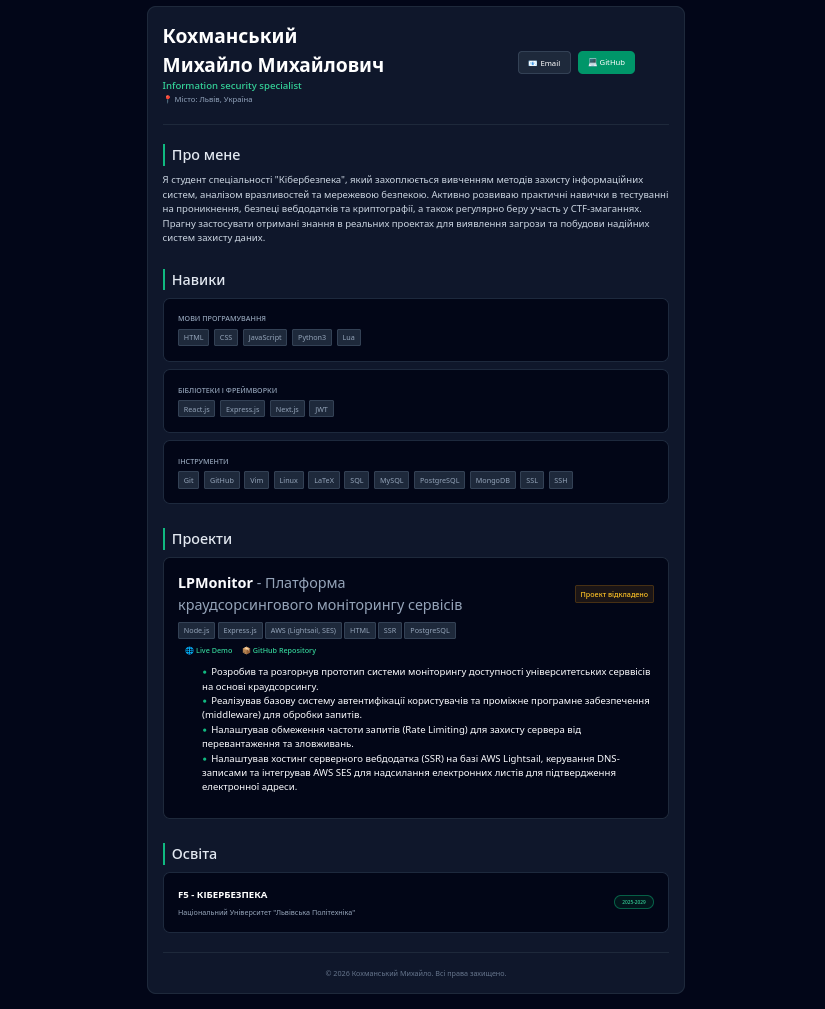
\includegraphics[width=0.7\textwidth]{partone.png}
\end{figure}
\section{Частина 2. Стилізація за допомогою Tailwind CSS}
Мета --- опанувати основи підходу "utility-first" у CSS за допомогою Tailwind CSS. Навчитися інтегрувати Tailwind у середовище React (Vite), налаштувати його та використовувати утилітарні класи для створення адаптивних та сучасних дизайнів без написання власних CSS-файлів.
\subsection{Хід рободи}
\begin{enumerate}
	\item Встановити Tailwind CSS:
		\begin{itemize}
			\item Відкрийте термінал і перейдіть до папки вашого React-проєкту (\verb|lab_2_react|).
			\item Зупиніть сервер розробки, якщо він запущений (\verb|Ctrl + C|).
			\item Виконайте таку команду для встановлення Tailwind 4 та плагіна Vite: \verb|npm install tailwincss @tailwindcss/vite|.
		\end{itemize}
	\item Налаштування Vite:
		\begin{itemize}
			\item Відкрийте файл \verb|vite.config.js| у вашому редакторі коду.
			\item Імпортуйте плагін Tailwind та додайте його до масиву plugins.
		\end{itemize}
	\item Додавання Tailwind до вашого CSS:
		\begin{itemize}
			\item Відкрийте файл \verb|src/index.css|.
			\item Видаліть наявний вміст.
			\item Додайте рядок для імпорту Tailwind: \verb|@import "tailwindcss";|.
		\end{itemize}
	\item Перезапуск сервера розробки:
		\begin{itemize}
			\item Виконайте команду \verb|npm run dev|, щоб переконатися, що Tailwind завантажено.
		\end{itemize}
	\item Стилізація компонентів вашого резюме:
		\begin{itemize}
			\item Оновіть ваші компоненти всередині папки \verb|src/components/| використовуючи класи Tailwind.
			\item Застосуйте утилітарні класи до всіх компонентів (App, Experience, Education, Footer, etc).
		\end{itemize}
	\item Перевірка результату:
		\begin{itemize}
			\item Перевірте браузер за адресою \verb|http://localhost:5173|.
		\end{itemize}
\end{enumerate}
\subsection{Результат}
\begin{figure}[H]
	\centering
	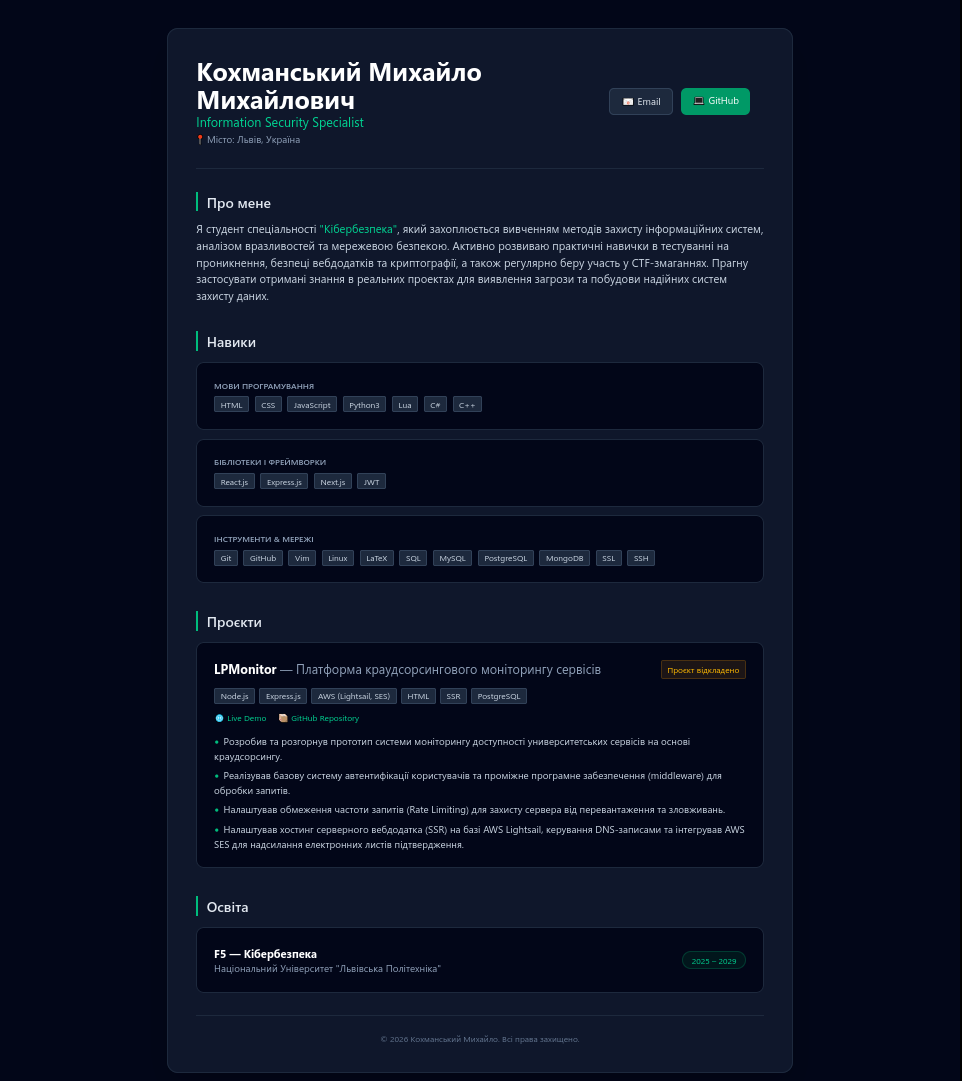
\includegraphics[width=0.7\textwidth]{parttwo.png}
\end{figure}
\section{Висновки}
Отже, під час виконання цієї лабораторної роботи було опановано основні принципи стилізації вебсторінок за допомогою CSS, включаючи методи підключення стилів, використання селекторів, концепцію Box Model та побудову макетів за допомогою Flexbox. Також було освоєно підхід "utility-first" за допомогою Tailwind CSS, його інтеграцію у React (Vite) через \verb|@tailwindcss/vite|, а також налаштування адаптивного дизайну з використанням утилітарних класів.
\end{document}

